\documentclass[aspectratio=169,10pt]{beamer}

\usetheme{default}
\useinnertheme{rectangles}
\setbeamertemplate{navigation symbols}{}
\setbeameroption{hide notes}
\setbeamersize{text margin left=0.7cm, text margin right=0.7cm}

\usepackage{amsmath,amssymb}
\usepackage[T1]{fontenc}
\usepackage[scaled=0.96]{FiraSans}
\usepackage{newtxsf}
\renewcommand{\familydefault}{\sfdefault}
\usepackage{microtype}
\usepackage{booktabs}
\usepackage{graphicx}
\usepackage{animate}
\usepackage{tikz}
\usetikzlibrary{arrows.meta,positioning,calc}

% Slide measures are short: avoid mid-word hyphenation.
\hyphenpenalty=10000
\exhyphenpenalty=10000

\definecolor{ink}{HTML}{202121}
\definecolor{forest}{HTML}{0E3B2C}
\definecolor{gold}{HTML}{D8AD62}
\definecolor{gilt}{HTML}{9E7B38}
\definecolor{paper}{HTML}{F4EFE3}
\definecolor{mist}{HTML}{C9CBC7}
\definecolor{muted}{HTML}{60645F}
\definecolor{clay}{HTML}{B04A2F}
\definecolor{orderedblue}{HTML}{3A6EA5}

\setbeamercolor{normal text}{fg=ink,bg=paper}
\setbeamercolor{background canvas}{bg=paper}
\setbeamercolor{frametitle}{fg=forest}
\setbeamercolor{structure}{fg=forest}
\setbeamercolor{block title}{fg=white,bg=forest}
\setbeamercolor{block body}{fg=ink,bg=paper!85!mist}
\setbeamercolor{itemize item}{fg=gilt}
\setbeamertemplate{itemize item}{\raisebox{0.15em}{\tiny$\blacktriangleright$}}
\setlength{\abovedisplayskip}{0.4em}
\setlength{\belowdisplayskip}{0.4em}

\newcommand{\relu}{\mathrm{ReLU}}
\newcommand{\E}{\mathbb{E}}
\newcommand{\cmulogo}{assets/logos/Carnegie_Mellon_University_seal.svg-2.png}
\newcommand{\iaifilogo}{assets/logos/IAIFI-logo-black.pdf}
\newcommand{\regularbackground}{assets/iaifi_regular_background.png}

% Consolidate the recurring header into one background object. This prevents
% PDF animation layers from selectively hiding its individual components.
\setbeamertemplate{background canvas}{%
  \includegraphics[width=\paperwidth,height=\paperheight]{\regularbackground}%
}
% Draw regular-slide chrome in the shipout foreground. This keeps it outside
% animation optional-content groups and above any opaque imported figures.
\makeatletter
\AddToHook{shipout/foreground}{%
  \ifbeamer@plainframe\else
    \begin{tikzpicture}[remember picture,overlay]
      \node[anchor=north east]
        at ($(current page.north east)+(-0.62cm,-0.15cm)$)
        {\includegraphics[height=1.05cm]{\cmulogo}};
      \draw[gold,line width=1.2pt]
        ($(current page.north west)+(0.70cm,-1.14cm)$) --
        ($(current page.north west)+(3.30cm,-1.14cm)$);
      \node[anchor=south west,text=muted,font=\scriptsize]
        at ($(current page.south west)+(0.70cm,0.10cm)$)
        {Lucas Fernandez-Sarmiento};
      \node[anchor=south,text=muted,font=\scriptsize]
        at ($(current page.south)+(0,0.10cm)$)
        {IAIFI Workshop 2026};
      \node[anchor=south east,text=muted,font=\scriptsize]
        at ($(current page.south east)+(-0.70cm,0.10cm)$)
        {\insertframenumber};
    \end{tikzpicture}%
  \fi
}
\makeatother
\newcommand{\regularpagechrome}{}
\newcommand{\localocgfallback}[1]{%
  % Some static PDF renderers mis-assign shared Beamer chrome to animation
  % optional-content groups. Redrawing these elements locally is harmless in
  % conforming viewers and keeps static handouts complete.
  \begin{tikzpicture}[remember picture,overlay]
    \if\relax\detokenize{#1}\relax\else
      % Mask the native title first: a few renderers expose only fragments of
      % it when the page follows an animation optional-content group.
      \fill[paper]
        ($(current page.north west)+(0.42cm,-0.10cm)$) rectangle
        ($(current page.north east)+(-1.42cm,-0.86cm)$);
      \node[anchor=west,text=forest,font=\bfseries\large]
        at ($(current page.north west)+(0.70cm,-0.47cm)$) {#1};
    \fi
    \node[anchor=north east]
      at ($(current page.north east)+(-0.62cm,-0.15cm)$)
      {\includegraphics[height=1.05cm]{\cmulogo}};
    \draw[gold,line width=1.2pt]
      ($(current page.north west)+(0.70cm,-1.14cm)$) --
      ($(current page.north west)+(3.30cm,-1.14cm)$);
    \node[anchor=south west,text=muted,font=\scriptsize]
      at ($(current page.south west)+(0.70cm,0.10cm)$)
      {Lucas Fernandez-Sarmiento};
    \node[anchor=south,text=muted,font=\scriptsize]
      at ($(current page.south)+(0,0.10cm)$)
      {IAIFI Workshop 2026};
  \end{tikzpicture}%
  \vspace*{-\baselineskip}% The overlay should not consume a content line.
}
\setbeamertemplate{background}{}

% Custom frame title: forest text on paper background, gold underline.
\setbeamertemplate{frametitle}{%
  \nointerlineskip
  \vspace{0.20cm}
  \hbox to \textwidth{%
    \vbox to 0.60cm{\vfil
      \hbox{{\color{forest}\bfseries\large\insertframetitle}}%
      \vfil}%
    \hfill%
  }%
  \vspace{0.03cm}
  \hbox to \textwidth{%
    \rule{0pt}{1.2pt}\hfill%
  }%
  \vspace{0.08cm}
}

% Reserve footer height on all non-plain slides.
\setbeamertemplate{footline}{%
  \leavevmode
  \hbox to \paperwidth{\rule[-0.11cm]{0pt}{0.36cm}\hfill}%
}

\title[Dropout Universality]{Dropout Universality}
\subtitle{Scaling Laws and Optimal Scheduling at the Edge-of-Chaos}
\author{Lucas Fernandez-Sarmiento}
\institute{Carnegie Mellon University}
\date{August 12, 2026}

\begin{document}

% -------------------------------------------------------------------------
% 1. Title
% -------------------------------------------------------------------------
\begin{frame}[plain]
  \begin{tikzpicture}[remember picture,overlay]
    \fill[paper] (current page.south west) rectangle (current page.north east);
    \draw[gold,line width=0.8pt]
      ($(current page.north west)+(0.75,-2.22)$) --
      ($(current page.north east)+(-0.75,-2.22)$);
    \node[anchor=north west] at ($(current page.north west)+(0.75,-0.38)$)
      {\includegraphics[height=1.02cm]{\iaifilogo}};
    \node[anchor=west,text=forest] at ($(current page.north west)+(1.88,-0.87)$)
      {\bfseries 2026 IAIFI Summer Workshop};
    \node[anchor=north east] at ($(current page.north east)+(-0.62,-0.18)$)
      {\includegraphics[height=2.05cm]{\cmulogo}};
  \end{tikzpicture}

  \vspace{2.48cm}
  \begin{center}
    {\color{ink}\bfseries\fontsize{22}{27}\selectfont
    Dropout Universality}\\[0.35em]
    {\color{forest}\fontsize{15}{19}\selectfont
    Scaling Laws and Optimal Scheduling at the Edge-of-Chaos}

    \vspace{0.65cm}
    {\color{gold}\rule{6.0cm}{1.0pt}}

    \vspace{0.48cm}
    {\Large\color{ink} Lucas Fernandez-Sarmiento}\\[0.18em]
    {\large\color{muted} Carnegie Mellon University}

    \vspace{0.28cm}
    {\small\color{forest}\bfseries Based on the ICML 2026 main-track paper}\\[0.10em]
    {\scriptsize\color{muted}
      \href{https://arxiv.org/abs/2605.21648}{Paper: arXiv:2605.21648}
      \(\cdot\)
      \href{https://icml.cc/virtual/2026/poster/65205}{ICML virtual poster 65205}}

    \vfill
    {\color{muted}August 12, 2026 \(\cdot\) MIT \(\cdot\) Cambridge, MA}
    \vspace{0.4cm}
  \end{center}
  \regularpagechrome
  \note{[Sources] Event details: \url{https://iaifi.org/summer-workshop.html}. Official IAIFI black logo: \url{https://iaifi.org/images/iaifi-logo-black.pdf}. Paper title, sole authorship, and ICML 2026 acceptance: \url{https://arxiv.org/abs/2605.21648}. ICML main-track virtual poster record: \url{https://icml.cc/virtual/2026/poster/65205}.}
\end{frame}

% -------------------------------------------------------------------------
% 2. Motivation: elephant
% -------------------------------------------------------------------------
\begin{frame}{Millions of weights are the wrong variables}
  \begin{columns}[c,onlytextwidth]
    \begin{column}{0.60\textwidth}
      \vspace{0.35em}
      {\color{ink}\itshape\fontsize{11}{14}\selectfont
      ``With four parameters I can fit an elephant, and with five I can make him wiggle his trunk.''}\\[0.35em]
      {\color{gilt}\small von Neumann to Fermi, via Dyson}

      \vspace{1.0em}
      
\begin{tikzpicture}
        \node[
          fill=forest!10!paper,
          fill opacity=0.45,
          draw=forest,
          line width=0.9pt,
          text opacity=1,
          text=ink,
          rounded corners=5pt,
          inner xsep=0.35cm,
          inner ysep=0.25cm,
          text width=0.88\linewidth,
          align=left
        ] {Can a few collective variables describe what depth does to information?};
      \end{tikzpicture}
    \end{column}

    \begin{column}{0.36\textwidth}
      \centering
      \animategraphics[method=icon,autoplay,loop,poster=first,width=0.96\linewidth,type=png]%
        {20}{assets/elephant_frames/elephant_}{0}{59}\\[0.35em]
      {\fontsize{4.8}{5.6}\selectfont\color{muted}
      Mayer, Khairy \& Howard\\
      Am.\ J.\ Phys.\ \textbf{78}, 648 (2010)}
    \end{column}
  \end{columns}
  \regularpagechrome
  \note{[Sources] Dyson, ``A meeting with Enrico Fermi,'' Nature 427, 297 (2004). Elephant construction: Mayer, Khairy \& Howard, Am. J. Phys. 78, 648 (2010).}
\end{frame}

% -------------------------------------------------------------------------
% 3. Broken-telephone mental model
% -------------------------------------------------------------------------
\begin{frame}{At initialization, depth is a broken telephone}
  \begingroup
  \small
  \begin{center}
    The same randomly initialized network retransmits two messages, layer after layer.
  \end{center}

  \vspace{0.10em}
  \begin{center}
  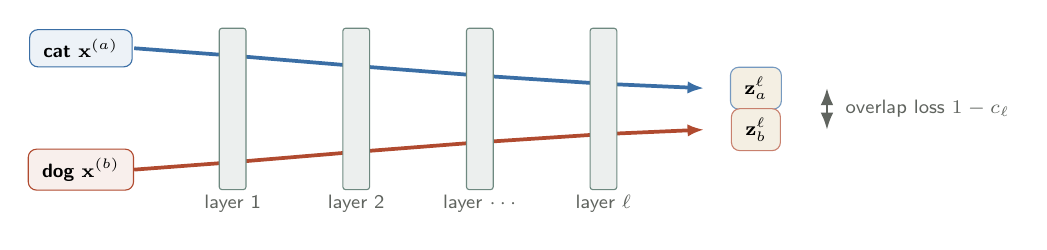
\begin{tikzpicture}[x=1cm,y=1cm,>=Latex,scale=0.94]
    % Draw the two signal paths first so the layer bars sit above them.
    \draw[orderedblue,line width=1.35pt,-{Latex[length=2.1mm]}]
      (0.72,0.82)--(2.05,0.72)--(3.72,0.58)--(5.39,0.45)--(7.06,0.34)--(8.42,0.28);
    \draw[clay,line width=1.35pt,-{Latex[length=2.1mm]}]
      (0.72,-0.82)--(2.05,-0.72)--(3.72,-0.58)--(5.39,-0.45)--(7.06,-0.34)--(8.42,-0.28);

    \foreach \x/\lab in {2.05/1,3.72/2,5.39/{\(\cdots\)},7.06/{\(\ell\)}} {
      \node[draw=forest!60,fill=forest!8,minimum width=0.34cm,
            minimum height=2.05cm,rounded corners=1pt] at (\x,0) {};
      \node[font=\scriptsize\color{muted}] at (\x,-1.28) {layer \lab};
    }

    \node[rounded corners=3pt,draw=orderedblue,fill=orderedblue!9,
          font=\bfseries\scriptsize,inner xsep=5pt,minimum width=1.30cm]
          at (0,0.82) {cat \(\mathbf x^{(a)}\)};
    \node[rounded corners=3pt,draw=clay,fill=clay!9,
          font=\bfseries\scriptsize,inner xsep=5pt,minimum width=1.30cm]
          at (0,-0.82) {dog \(\mathbf x^{(b)}\)};
    \node[rounded corners=3pt,draw=orderedblue!70,fill=paper,
          font=\scriptsize,inner xsep=5pt] at (9.12,0.28) {\(\mathbf z_a^\ell\)};
    \node[rounded corners=3pt,draw=clay!70,fill=paper,
          font=\scriptsize,inner xsep=5pt] at (9.12,-0.28) {\(\mathbf z_b^\ell\)};
    \draw[<->,muted,line width=0.7pt] (10.08,0.28)--(10.08,-0.28);
    \node[anchor=west,font=\scriptsize\color{muted}] at (10.20,0) {overlap loss \(1-c_\ell\)};
  \end{tikzpicture}
  \end{center}

  \vspace{0.10em}
  \begin{columns}[c,onlytextwidth]
    \begin{column}{0.59\textwidth}
      \[
        c_\ell=
        \frac{\langle \mathbf z_a^\ell,\mathbf z_b^\ell\rangle}
        {\|\mathbf z_a^\ell\|\,\|\mathbf z_b^\ell\|}
      \]
    \end{column}
    \begin{column}{0.37\textwidth}
      {\color{forest}\bfseries Track how much of their distinction survives---not every microscopic weight.}
    \end{column}
  \end{columns}

  \vspace{0.12em}
  {\scriptsize\color{muted}Weights are sampled once and shared by both inputs; conditioned on them, the forward map is deterministic. Here \(c_\ell\) is representation overlap, not semantic similarity or accuracy.}
  \endgroup
  \regularpagechrome
  \note{[Sources] Broken telephone is a presenter analogy. Random-network signal propagation and normalized overlap: Poole et al., NeurIPS 2016; Schoenholz et al., ICLR 2017; paper Sec. 2.}
\end{frame}

% -------------------------------------------------------------------------
% 4. Correlation problem and criticality cartoon
% -------------------------------------------------------------------------
\begin{frame}{Initialization controls how long information survives}
  \localocgfallback{}
  \begingroup
  \small
  \begin{center}
    Follow the normalized overlap \(c_\ell\) as depth grows.
  \end{center}

  \vspace{0.10em}
  \begin{columns}[T,onlytextwidth]
    \begin{column}{0.31\textwidth}
      \centering
      {\color{orderedblue}\bfseries Ordered}\\[0.15em]
      \(c_\ell\to1\) quickly\\
      normalized representations align
    \end{column}
    \begin{column}{0.31\textwidth}
      \centering
      {\color{forest}\bfseries Critical edge}\\[0.15em]
      forgetting is slow\\
      distinctions survive many layers
    \end{column}
    \begin{column}{0.31\textwidth}
      \centering
      {\color{clay}\bfseries Chaotic}\\[0.15em]
      differences amplify initially\\
      then saturate at lower overlap
    \end{column}
  \end{columns}

  \vspace{0.28em}
  \begin{center}
    \animategraphics[method=icon,autoplay,loop,poster=first,width=0.63\textwidth,type=png]%
      {16}{assets/manifold_slide_frames_t/manifold_}{0}{200}

    \vspace{-0.12em}
    {\scriptsize\color{muted}A circular input manifold propagated through random \(\tanh\) layers and projected to 2D.}

    \vspace{0.12em}
    
\begin{tikzpicture}
      \node[draw=forest,fill=forest!8,rounded corners=5pt,
            inner xsep=0.42cm,inner ysep=0.22cm,text=ink]
        {Tune initialization to the edge so input distinctions propagate deepest.};
    \end{tikzpicture}
  \end{center}
  \endgroup
  \regularpagechrome
  \note{[Sources] Ordered, edge-of-chaos, and chaotic signal-propagation regimes: Poole et al., NeurIPS 2016; Schoenholz et al., ICLR 2017. Animation generated from the mean-field propagation setup documented with this deck.}
\end{frame}

% -------------------------------------------------------------------------
% 5. Mean-field assumptions
% -------------------------------------------------------------------------
\begin{frame}{Infinite width makes the moment dynamics deterministic}
  \begingroup
  \small
  \begin{columns}[T,onlytextwidth]
    \begin{column}{0.51\textwidth}
      {\color{forest}\bfseries Random fully connected layer}
      \begin{align*}
        z_{i;a}^{\ell+1}
          &=\sum_{j=1}^{N}W_{ij}^{\ell+1}
            \phi\!\left(z_{j;a}^{\ell}\right)+b_i^{\ell+1},\\
        W_{ij}^{\ell}&\sim\mathcal N\!\left(0,\frac{\sigma_w^2}{N}\right),
        &b_i^{\ell}&\sim\mathcal N(0,\sigma_b^2).
      \end{align*}

      \vspace{0.15em}
      Each layer's matrix is sampled at initialization and then held fixed. Both inputs see the same matrices; there is no additive noise redrawn on each pass.
    \end{column}

    \begin{column}{0.45\textwidth}
      {\color{forest}\bfseries Mean-field assumptions}
      \begin{itemize}
        \setlength{\itemsep}{0.45em}
        \item width \(N\to\infty\),
        \item i.i.d. Gaussian initialization,
        \item a fixed activation \(\phi\),
        \item exchangeable neurons within a layer.
      \end{itemize}

      \vspace{0.35em}
      {\color{muted}Finite wide networks approximate this ensemble law.}
    \end{column}
  \end{columns}

  \vspace{0.40em}
  \begin{center}
    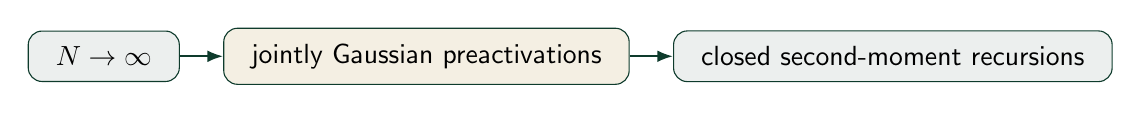
\begin{tikzpicture}[>=Latex]
      \node[draw=forest,fill=forest!8,rounded corners=5pt,
            inner xsep=0.35cm,inner ysep=0.20cm] (a)
        {\(N\to\infty\)};
      \node[right=0.55cm of a,draw=forest,fill=paper,rounded corners=5pt,
            inner xsep=0.35cm,inner ysep=0.20cm] (b)
        {jointly Gaussian preactivations};
      \node[right=0.55cm of b,draw=forest,fill=forest!8,rounded corners=5pt,
            inner xsep=0.35cm,inner ysep=0.20cm] (c)
        {closed second-moment recursions};
      \draw[forest,line width=0.8pt,-{Latex[length=2mm]}] (a)--(b);
      \draw[forest,line width=0.8pt,-{Latex[length=2mm]}] (b)--(c);
    \end{tikzpicture}
  \end{center}

  \vfill
  \begin{center}
    {\small\color{clay}\bfseries The limit is infinite width; depth \(\ell\) remains the iteration coordinate.}
  \end{center}
  \endgroup
  \regularpagechrome
  \note{[Sources] Neal, Bayesian Learning for Neural Networks (1996); Poole et al., NeurIPS 2016; Schoenholz et al., ICLR 2017; paper Sec. 2 and App. C.}
\end{frame}

% -------------------------------------------------------------------------
% 6. Closed recursions
% -------------------------------------------------------------------------
\begin{frame}{Infinite width closes on variance and overlap}
  \localocgfallback{Infinite width closes on variance and overlap}
  \begingroup
  \small
  \begin{columns}[T,onlytextwidth]
    \begin{column}{0.66\textwidth}
      The Gaussian second moments obey deterministic recursions:
      \begin{align*}
        q_{aa}^{\ell+1}
        &=\sigma_w^2\!\int Dz\,
          \phi^2\!\left(\sqrt{q_{aa}^{\ell}}z\right)+\sigma_b^2,\\[0.22em]
        q_{ab}^{\ell+1}
        &=\sigma_w^2\,\E_{(u_a,u_b)}
          \left[\phi(u_a)\phi(u_b)\right]+\sigma_b^2,\\[0.22em]
        c_{ab}^{\ell}
        &=\frac{q_{ab}^{\ell}}
          {\sqrt{q_{aa}^{\ell}q_{bb}^{\ell}}}.
      \end{align*}
      {\scriptsize\color{muted}\((u_a,u_b)\) are jointly Gaussian with covariance fixed by \(q_{aa}^{\ell},q_{bb}^{\ell},q_{ab}^{\ell}\), and \(Dz=e^{-z^2/2}dz/\sqrt{2\pi}\).}
    \end{column}

    \begin{column}{0.30\textwidth}
      {\color{forest}\bfseries Macroscopic variables}

      \vspace{0.45em}
      \(q^\ell\): signal scale

      \vspace{0.45em}
      \(c^\ell\): normalized cat--dog representation overlap

      \vspace{0.55em}
      Once \(q^\ell\to q^*\),
      \[
        \boxed{c_{\ell+1}=F(c_\ell)}
      \]

      \vspace{0.25em}
      {\scriptsize At equal variance,
      \(\E\|\mathbf z_a-\mathbf z_b\|^2/N=2q^*(1-c)\).}
    \end{column}
  \end{columns}

  \vfill
  \begin{center}
    {\color{forest}\bfseries Millions of weights have become a one-dimensional dynamical system in depth.}
  \end{center}
  \endgroup
  \localocgfallback{}
  \regularpagechrome
  \note{[Sources] Poole et al., NeurIPS 2016; Schoenholz et al., ICLR 2017; paper Sec. 2 and App. C. The squared-distance identity follows directly from equal variances and normalized covariance.}
\end{frame}

% -------------------------------------------------------------------------
% 7. Linearization and correlation depth
% -------------------------------------------------------------------------
\begin{frame}{A fixed point is not the same as criticality}
  \begingroup
  \small
  \begin{columns}[T,onlytextwidth]
    \begin{column}{0.43\textwidth}
      {\color{forest}\bfseries Destination}
      \[
        c^*=F(c^*)
      \]

      {\color{forest}\bfseries Linearized approach}
      \begin{align*}
        \delta c_{\ell+1}&\simeq\lambda\,\delta c_\ell,
        &\lambda&=F'(c^*),\\
        |c_\ell-c^*|&\simeq|c_0-c^*|e^{-\ell/\xi_c},
        &\xi_c^{-1}&=-\log|\lambda|.
      \end{align*}

      \vspace{0.15em}
      \begin{tabular}{@{}cl@{}}
        \(0\le\lambda<1\) & stable, finite \(\xi_c\) \\
        \(\lambda=1\) & marginal / critical edge \\
        \(\lambda>1\) & unstable
      \end{tabular}
    \end{column}

    \begin{column}{0.53\textwidth}
      \vspace{-1.00em}
      \begin{center}
        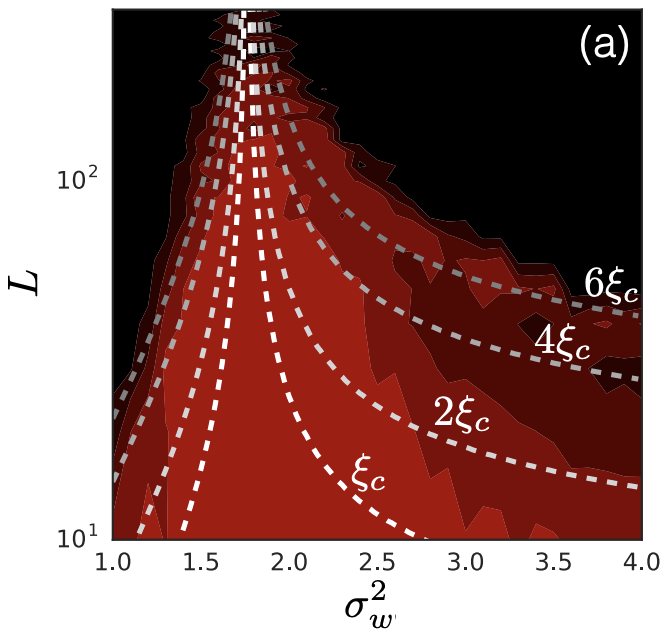
\includegraphics[height=0.52\textheight]{assets/dip_trainability_transparent.png}\\[-0.35em]
        {\tiny\color{muted}Schoenholz et al., \emph{Deep Information Propagation}, ICLR 2017}
      \end{center}
    \end{column}
  \end{columns}

  \vspace{-0.30em}
  \begin{center}
    
\begin{tikzpicture}
      \node[draw=forest,fill=forest!8,rounded corners=5pt,
            inner xsep=0.42cm,inner ysep=0.20cm,text=ink]
        {The fixed point says \emph{where} the network goes; the slope says \emph{how fast} it forgets.};
    \end{tikzpicture}
  \end{center}

  \vspace{0.08em}
  {\scriptsize\color{muted}Without dropout, \(c=1\) is always a fixed point and \(\chi_\perp\equiv F'(1)\); the edge is \(\chi_\perp=1\). Here \(\xi_c\) is an e-folding depth for forward overlap relaxation.}
  \endgroup
  \regularpagechrome
  \note{[Sources] Linearized correlation dynamics and trainability plot: Schoenholz et al., ICLR 2017; paper Sec. 2. For the no-dropout wide MLP, the same derivative-squared kernel controls mean-squared gradient scaling; this slide defines the forward depth scale.}
\end{frame}

% -------------------------------------------------------------------------
% 8. Curie--Weiss analogy and physics dictionary
% -------------------------------------------------------------------------
\begin{frame}{Curie--Weiss supplies a dictionary---not the universality class}
  \begingroup
  \footnotesize
  \begin{columns}[T,onlytextwidth]
    \begin{column}{0.43\textwidth}
      \centering
      {\small\color{forest}\bfseries Curie--Weiss magnet}
      \[
        M=\tanh\!\left[\beta(JM+H)\right]
      \]
      Many spins close on one self-consistent variable.

      \vspace{0.55em}
      {\small\color{forest}\bfseries Wide neural network}
      \[
        c_{\ell+1}=F(c_\ell),\qquad c^*=F(c^*)
      \]
      Many neurons close on one overlap map.
    \end{column}

    \begin{column}{0.53\textwidth}
      {\small\color{forest}\bfseries Effective variables and control parameters}

      \vspace{0.15em}
      \scriptsize
      \setlength{\tabcolsep}{3pt}
      \renewcommand{\arraystretch}{1.24}
      \begin{tabular}{@{}rcl@{}}
        \toprule
        \textbf{Curie--Weiss} & & \textbf{Wide network} \\
        \midrule
        magnetization \(M\) & \(\longleftrightarrow\) & \(m=1-c^*\) \\
        detuning \(\beta J-1\) & \(\longleftrightarrow\) & \(t=\chi_\rho-1\) \\
        external field \(H\) & \(\longleftrightarrow\) & \(h=1-\bar F_\rho(1)\) \\
        susceptibility & \(\longleftrightarrow\) & \(\chi_M=\partial m/\partial h\) \\
        correlation scale & \(\longleftrightarrow\) & \(\xi_c^{-1}=-\log|\bar F_\rho'(c^*)|\) \\
        \bottomrule
      \end{tabular}

      \vspace{0.55em}
      {\small\color{forest}\bfseries Microscopic controls}
      \[
        (\sigma_w^2,\,\sigma_b^2,\,\rho)
        \quad\longrightarrow\quad \bar F_\rho
      \]

      {\scriptsize\color{muted}\(\chi_\rho=\bar F_\rho'(1)\) is a map-slope detuning; \(\chi_M\) is a field-response susceptibility.}
    \end{column}
  \end{columns}

  \vfill
  \begin{center}
    {\small\color{clay}\bfseries Structural analogy only:}
    {\small depth is iteration, not equilibrium time or distance; \(m\ge0\) has no \(\mathbb Z_2\) symmetry.}
  \end{center}
  \endgroup
  \regularpagechrome
  \note{[Sources] Curie--Weiss self-consistency equation: standard mean-field Ising theory; see Landau \& Lifshitz, Statistical Physics. Neural dictionary and caveats: paper Sec. 3, App. B, and App. C.}
\end{frame}

% -------------------------------------------------------------------------
% 9. Visual introduction to dropout and displaced alignment
% -------------------------------------------------------------------------
\begin{frame}{Dropout randomly thins the network during training}
  \begingroup
  \vspace{0.10em}
  \begin{center}
    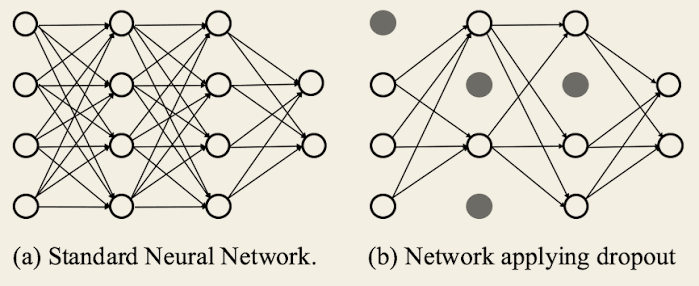
\includegraphics[width=0.78\textwidth]{assets/dropout_reference_paper.png}
  \end{center}

  \vspace{-0.10em}
  \begin{center}
    {\large Each training pass samples a different thinned network.}\\[0.16em]
    {\small Mean activation is rescaled back, but independent masks reduce pairwise alignment.}
  \end{center}

  \vfill
  {\scriptsize\color{muted}At inference all units return. Independent masks remove perfect alignment; weak dropout later appears as \(h\propto1-\rho\).}
  \endgroup
  \regularpagechrome
  \note{[Sources] Inverted dropout and training/inference behavior: Srivastava et al., JMLR 15, 1929 (2014). Diagram supplied by the presenter as ``images (2).png''; its geometry and labels are unchanged, with only the white background composited onto the deck's paper color. Independent-mask geometry, displaced fixed point, and weak-dropout field: paper Sec. 3 and App. D.}
\end{frame}

% -------------------------------------------------------------------------
% 10. Dropout field as a running coupling and schedule functional
% -------------------------------------------------------------------------
\begin{frame}{Depth is an RG scale; dropout makes the field run}
  \localocgfallback{}
  \begingroup
  \footnotesize
  \setlength{\abovedisplayskip}{0.14em}
  \setlength{\belowdisplayskip}{0.14em}

  \begin{center}
    {\large\bfseries
      network depth \(\ell\uparrow\)
      \(\longleftrightarrow\)
      QFT scale \(\mu\downarrow\) toward the infrared}

    \vspace{0.18em}
    {\small At criticality: \(\ell\to\infty\)
      \(\longrightarrow\) a scale-invariant, CFT-like fixed point.}

    \vspace{0.08em}
    {\tiny\color{muted}Representation-group analogy; generic MLPs are not thereby proven to be conformal.
    \enspace Roberts, Yaida \& Hanin, \emph{The Principles of Deep Learning Theory} (2022).}
  \end{center}

  \vspace{0.22em}
  {\color{forest}\bfseries Coarse-graining representations makes the effective coefficients run with depth.}

  \vspace{0.10em}
  \begin{center}
    \scriptsize
    \setlength{\tabcolsep}{5pt}
    \renewcommand{\arraystretch}{1.13}
    \begin{tabular}{@{}lll@{}}
      \toprule
      \textbf{coefficient} & \textbf{network definition} & \textbf{effective-theory role} \\
      \midrule
      \(t_\ell\) & \(\chi_{\rho_\ell}-1\) & temperature/mass-like detuning \\
      \(h_\ell\) & \(1-\bar F_{\rho_\ell}(1)\) & relevant decorrelation source \\
      \(g_\ell\) & \(\bar F_{\rho_\ell}''(1)\) & smooth analytic interaction \\
      \(\kappa_\ell\) & branch-point amplitude & kinked non-analytic interaction \\
      \bottomrule
    \end{tabular}
  \end{center}

  \vspace{0.18em}
  \begin{columns}[T,onlytextwidth]
    \begin{column}{0.62\textwidth}
      Let \(d(\ell)\equiv1-\rho(\ell)\) be the layerwise dropout rate. At the edge,
      \[
        \xi_{\mathrm{eff}}[d] =
        \left[\frac{A}{L}\int_0^L
        h\!\left(d(\ell)\right)^a\,\mathrm d\ell\right]^{-1},
        \qquad
        a=\begin{cases}\tfrac12&\text{smooth},\\[-0.12em]\tfrac13&\text{kinked}.\end{cases}
      \]
      \[
        \frac{\delta\,\xi_{\mathrm{eff}}^{-1}}{\delta d(\ell)}
        =\frac{Aa}{L}\,h(d)^{a-1}\frac{\mathrm dh}{\mathrm dd}
        \quad\xrightarrow[\int d=\mathrm{const.}]{\ 0\le d\le d_{\max}\ }
        \quad\text{saturated schedules.}
      \]
    \end{column}

    \begin{column}{0.34\textwidth}
      
\begin{tikzpicture}
        \node[draw=gold,fill=gold!12,rounded corners=4pt,
              text width=0.87\linewidth,align=center,inner sep=6pt]
          {\bfseries\color{forest}Dropout makes the source explicit\\[0.25em]
           \normalfont\(h[d]=A_1d+\mathcal O(d^2)\)\\[0.35em]
           \(\Downarrow\)\\[0.25em]
           \bfseries depth-dependent\\dropout schedules};
      \end{tikzpicture}
    \end{column}
  \end{columns}

  \vfill
  {\tiny\color{muted}The propagation functional is permutation invariant; regularization reach selects the earliest placement on the next slide.}
  \endgroup
  \regularpagechrome
  \note{[Sources] Representation-group flow and the effective-theory/RG interpretation of depth: Roberts, Yaida, and Hanin, The Principles of Deep Learning Theory (Cambridge University Press, 2022), especially Ch. 4; arXiv:2106.10165. The depth--energy correspondence shown is an RG-scale analogy: increasing depth corresponds to coarse-graining toward the infrared, and the CFT-like endpoint is only the scale-invariant critical analogue. Field definition, weak-dropout expansion, correlation-depth functional, activation-dependent powers, variational derivative, and scheduling constraints: paper Secs. 3.1 and 4 and Apps. D--E. The propagation functional is permutation invariant; regularization reach motivates early placement.}
\end{frame}

% -------------------------------------------------------------------------
% 11. Scaling collapse and 1PI effective-action interpretation
% -------------------------------------------------------------------------
\begin{frame}{Critical data collapse onto one universal curve}
  \begingroup
  \centering
  \vspace{-0.20em}
  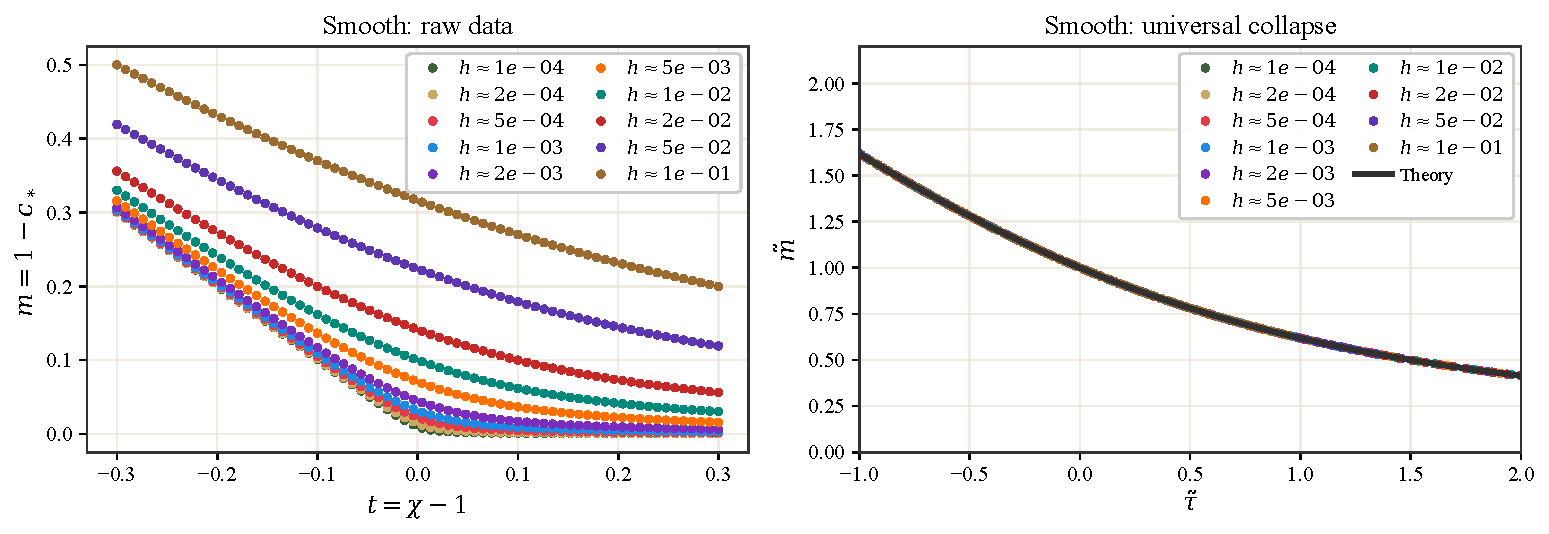
\includegraphics[width=0.695\textwidth]{../figures/theory/smooth_scaling_collapse.pdf}

  \vspace{-0.30em}
  \begin{columns}[T,onlytextwidth]
    \begin{column}{0.47\textwidth}
      \scriptsize
      {\color{forest}\bfseries Two parameters become one scaling variable}
      \[
        \begin{aligned}
          m_s(t,h)&=h^{1/2}\mathcal M_s(t/h^{1/2}),\\[-0.12em]
          m_k(t,h)&=h^{2/3}\mathcal M_k(t/h^{1/3}).
        \end{aligned}
      \]
      {\tiny\color{muted}Smooth normal form:
      \(\tilde m=\sqrt{1+\tilde t^2}-\tilde t\),
      \(\tilde m=m\sqrt{g_\rho/(2h)}\),
      \(\tilde t=-t/\sqrt{2g_\rho h}\).}
    \end{column}

    \begin{column}{0.49\textwidth}
      \scriptsize
      {\color{forest}\bfseries The field-theory reading}

      Connected \(n\)-point correlators are homogeneous at criticality and
      collapse after rescaling by their critical dimensions; 1PI vertices
      inherit conjugate scaling after the Legendre transform.

      \vspace{0.10em}
      Both equations of state follow from a reduced (zero-momentum) 1PI action:
      \[
        \begin{aligned}
          \Gamma_{\mathrm{eff}}&=-\frac{t}{2}m^2+\mathcal V(m)-hm,
          &\partial_m\Gamma_{\mathrm{eff}}&=0,\\[-0.10em]
          \mathcal V_s&=\frac{g_\rho}{6}m^3,
          &\mathcal V_k&=\frac{2\kappa}{5}m^{5/2}.
        \end{aligned}
      \]
    \end{column}
  \end{columns}

  \vspace{-0.40em}
  {\tiny\color{muted}Reduced Landau/1PI action only---not the training loss and not derived from a neural partition function.}
  \endgroup
  \regularpagechrome
  \note{[Sources] Two-parameter collapse, rescaled variables, and figure: paper Sec. 3.1, ``Scaling Collapse and Crossover Region,'' and Fig. 3; the curves are generated from the full mean-field recursions. Homogeneous scaling of connected n-point functions and corresponding 1PI vertex functions after the Legendre transform: Zinn-Justin, Quantum Field Theory and Critical Phenomena (2002). The reduced effective-action interpretation and its caveats follow paper App. D.}
\end{frame}

% -------------------------------------------------------------------------
% 12. Scheduling theory
% -------------------------------------------------------------------------
\begin{frame}[t]{Concavity concentrates dropout; reach puts it early}
  \begingroup
  \begin{columns}[T,onlytextwidth]
    \begin{column}{0.50\textwidth}
      \small
      At the correlation edge in the weak-field regime,
      \vspace{-0.15em}
      \[
        \xi_{\mathrm{eff}}^{-1}
        \propto \frac{1}{L}\sum_{\ell=1}^{L}h_\ell^a,
        \qquad
        a=\begin{cases}
          \tfrac12 & \text{smooth},\\
          \tfrac13 & \text{kinked}.
        \end{cases}
      \]
      \vspace{-0.25em}
      Fixed field budget and local bound:
      \vspace{-0.15em}
      \[
        \frac1L\sum_\ell h_\ell=\bar h,
        \qquad 0\le h_\ell\le h_{\max}.
      \]

      \vspace{-0.2em}
      \begin{itemize}
        \setlength{\itemsep}{0.15em}
        \item Concavity + bound \(\Rightarrow\) saturated blocks.
        \item Propagation is indifferent to layer order.
        \item Earlier masks influence a longer downstream suffix.
      \end{itemize}
    \end{column}

    \begin{column}{0.46\textwidth}
      \centering
      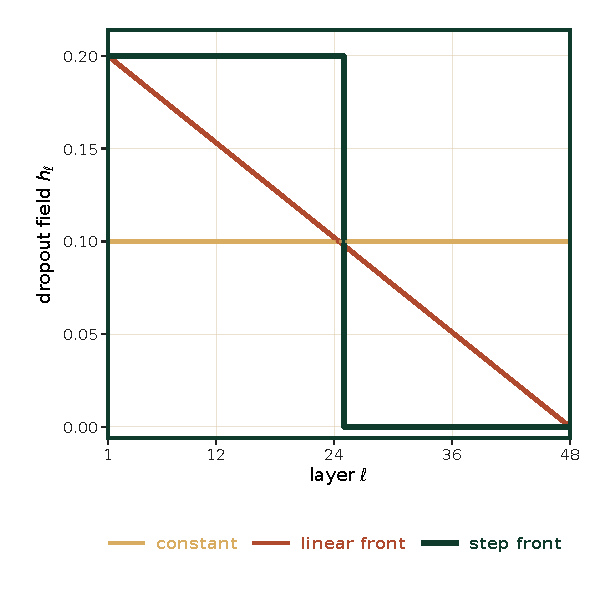
\includegraphics[width=0.84\linewidth]{assets/results/frontloaded_schedule_comparison.pdf}
    \end{column}
  \end{columns}
  \endgroup
  \regularpagechrome
  \note{[Sources] Paper Sec. 4, ``Optimal Dropout Scheduling and Regularization Reach.'' The field-budget and raw dropout-budget statements agree to leading order at weak dropout. Schedule figure generated from the paper's fixed-budget profiles.}
\end{frame}

% -------------------------------------------------------------------------
% 13. Empirical validation
% -------------------------------------------------------------------------
\begin{frame}{Front-loading improves quality---and reaches it sooner}
  % Local foreground fallback: Quartz can suppress the shared header object on
  % this imported-PDF page when animation OCGs are present elsewhere.
  \begin{tikzpicture}[remember picture,overlay]
    \node[anchor=north east]
      at ($(current page.north east)+(-0.62cm,-0.15cm)$)
      {\includegraphics[height=1.05cm]{\cmulogo}};
    \draw[gold,line width=1.2pt]
      ($(current page.north west)+(0.70cm,-1.14cm)$) --
      ($(current page.north west)+(3.30cm,-1.14cm)$);
  \end{tikzpicture}
  \begin{columns}[c,onlytextwidth]
    \begin{column}{0.55\textwidth}
      \centering
      {\color{forest}\bfseries Best test accuracy across schedules}\\[0.10em]
      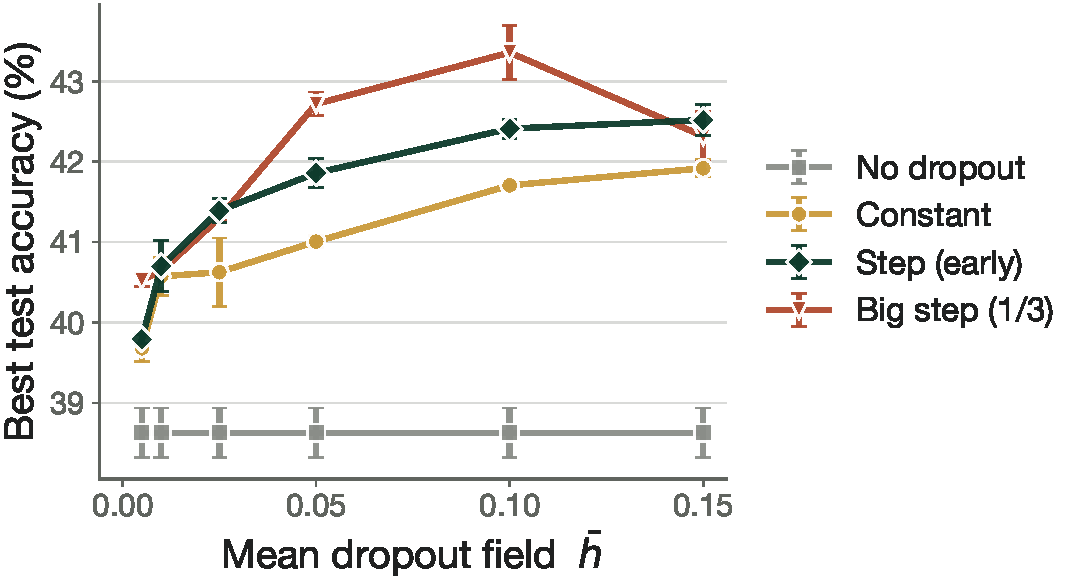
\includegraphics[width=0.92\linewidth]{assets/results/h_sweep_schedule_styled.pdf}
    \end{column}

    \begin{column}{0.41\textwidth}
      \centering
      {\color{forest}\bfseries Final-epoch test-loss reduction}

      \vspace{0.20em}
      {\fontsize{21}{24}\selectfont\color{forest}\bfseries 18--35\%}\\[-0.05em]
      {\normalsize MLP settings}

      \vspace{0.25em}
      {\color{gold}\rule{4.2cm}{1.0pt}}

      \vspace{0.25em}
      {\fontsize{21}{24}\selectfont\color{forest}\bfseries 4--6\%}\\[-0.05em]
      {\normalsize Vision Transformers}

      \vspace{0.25em}
      {\color{gold}\rule{4.2cm}{1.0pt}}

      \vspace{0.25em}
      {\color{forest}\bfseries Time to uniform-dropout final accuracy}\\[0.05em]
      {\fontsize{21}{24}\selectfont\color{clay}\bfseries \(\sim\!60\%\) less compute}\\[-0.05em]
      {\normalsize 29--31 versus 75 epochs}

      \vspace{0.24em}
      {\tiny Primary CIFAR-10 \(\relu\) MLP, \(\bar h=0.1\), equal per-epoch cost.\\
      Loss ranges use fixed- or matched-budget constant-dropout baselines.}
    \end{column}
  \end{columns}
  \note{[Sources] Paper App. H and Table 5. Exact final-epoch relative cross-entropy reductions: MLP 17.9, 22.6, 35.4, 29.8 percent; ViT 4.2, 6.3 percent. Plot: paper h-sweep data restyled for this deck. Time-to-target compute is calculated from the archived primary ReLU MLP scheduling experiment at mean field budget hbar=0.1 (25 simulations, 75 epochs). The constant/uniform schedule's ensemble-mean final test accuracy is 41.84 percent. Step (early) first exceeds and thereafter remains above that target at epoch 31, while Big step (1/3) does so at epoch 29. The corresponding epoch savings are 1-31/75=58.7 percent and 1-29/75=61.3 percent, summarized visibly as approximately 60 percent. Architecture, batch size, and epoch definition are identical, so this is epoch-proportional training compute to a fixed accuracy target, not a reduction in per-step FLOPs or measured wall-clock time.}
\end{frame}

% -------------------------------------------------------------------------
% 14. Close
% -------------------------------------------------------------------------
\begin{frame}[plain]
  \begin{tikzpicture}[remember picture,overlay]
    \fill[paper] (current page.south west) rectangle (current page.north east);
    \node[anchor=north west] at ($(current page.north west)+(0.75,-0.38)$)
      {\includegraphics[height=0.82cm]{\iaifilogo}};
    \node[anchor=north east] at ($(current page.north east)+(-0.30,-0.18)$)
      {\includegraphics[height=1.85cm]{\cmulogo}};
  \end{tikzpicture}

  \vspace{1.15cm}
  \begin{center}
    \resizebox{0.70\paperwidth}{!}{%
      \color{forest}\bfseries From microscopic masks to a macroscopic design rule}

    \vspace{0.52cm}
    {\Large Dropout is an external field.}\\[0.25em]
    {\color{gold}\Large\(\Downarrow\)}\\[0.20em]
    {\Large Activation analyticity selects the universality class.}\\[0.25em]
    {\color{gold}\Large\(\Downarrow\)}\\[0.20em]
    {\Large\color{forest}\bfseries At fixed budget, put the field early.}

    \vspace{0.45cm}
    {\color{gold}\rule{6.5cm}{1.0pt}}

    \vspace{0.35cm}
    {\small\color{muted}Outlook: treat other depth-dependent hyperparameters as dynamical fields.}

    \vspace{0.32cm}
    {\large\color{forest}\bfseries Questions?}\\[0.15em]
    {\scriptsize\color{muted}Lucas Fernandez-Sarmiento \(\cdot\) Carnegie Mellon University \(\cdot\) IAIFI Workshop 2026}
  \end{center}
  \regularpagechrome
  \note{[Sources] Synthesis of the paper's main theoretical and empirical conclusions; outlook matches the submitted IAIFI workshop abstract at \url{https://iaifi.org/summer-workshop.html}.}
\end{frame}

% -------------------------------------------------------------------------
% 15. Backup exponent dictionary
% -------------------------------------------------------------------------
\begin{frame}{Backup: the complete critical-exponent dictionary}
  \begin{center}
    \small
    \setlength{\tabcolsep}{3.5pt}
    \renewcommand{\arraystretch}{1.10}
    \begin{tabular}{@{}lccccccc@{}}
      \toprule
      Universality class & \(\nu_t\) & \(\beta\) & \(\theta_{\rm rel}\) & \(\gamma\) & \(\delta\) & \(\nu_\rho\) & \(\alpha\) \\
      \midrule
      Smooth activation & \(1\) & \(1\) & \(1\) & \(1\) & \(2\) & \(\tfrac12\) & \(-1\) \\
      Kinked activation & \(1\) & \(2\) & \(2\) & \(1\) & \(\tfrac32\) & \(\tfrac13\) & \(-3\) \\
      Spin glass (SK MF) & \(\tfrac12\) & \(1\) & \(2\) & \(1\) & \(2\) & \(\tfrac14\) & \(-1\) \\
      Ising-like (Landau MF) & \(\tfrac12\) & \(\tfrac12\) & \(1\) & \(1\) & \(3\) & \(\tfrac13\) & \(0\) \\
      \bottomrule
    \end{tabular}
  \end{center}

  \vspace{0.30em}
  \begin{columns}[T,onlytextwidth]
    \begin{column}{0.48\textwidth}
      \small
      \setlength{\jot}{1.5pt}
      \begin{align*}
        m&\sim |t|^\beta &&(h=0),\\
        m&\sim |h|^{1/\delta} &&(t=0),\\
        \chi_M&\sim |t|^{-\gamma},\\
        C&\sim |t|^{-\alpha}.
      \end{align*}
    \end{column}
    \begin{column}{0.48\textwidth}
      \small
      \setlength{\jot}{1.5pt}
      \begin{align*}
        \xi&\sim |t|^{-\nu_t} &&(h=0),\\
        \xi&\sim |h|^{-\nu_\rho} &&(t=0),\\
        m_\ell&\sim \ell^{-\theta_{\rm rel}} &&(t=h=0).
      \end{align*}
    \end{column}
  \end{columns}

  \vspace{0.20em}
  {\scriptsize\color{muted}The kinked \(\nu_\rho\) is a normal-form field exponent. Ordinary bias-free \(\relu\) follows the constrained path \(t=-h\) and retains \(\xi\sim h^{-1/3}\).}
  \regularpagechrome
  \note{[Sources] Paper Table 1 and App. D, complete exponent definitions and derivations.}
\end{frame}

\end{document}
